\subsection{Data Fetching and Feature Extraction}
\label{subsec:results_data}

The results section commences with the presentation of Table~\ref{tab:records}, which summarizes the data retrieval phase.
Displayed within are the total records obtained from both databases, along with the corresponding total and median values extracted.

\begin{table}
    \renewcommand{\arraystretch}{1.5}
    \setlength{\tabcolsep}{12pt}
    \begin{center}
        \begin{tabular}{ |c|c|c| }
            \hline
            & MIMIC-III  & MIMIC-IV  \\
            \hline
            Records       & 22,083     & 5,508     \\
            \hline
            Total Values  & 13,659,375 & 1,309,265 \\
            \hline
            Median Values & 1,918,623  & 183,140   \\
            \hline
        \end{tabular}
    \end{center}
    \captionsetup{format=plain, justification=centering}
    \caption{Fetched and Extracted Data from MIMIC-III and MIMIC-IV DBs}
    \label{tab:records}
\end{table}

In a brief summary of the table data, 5,508 records were retrieved from the MIMIC-IV database, each encompassing 37,795 values, equating to approximately 605 seconds of data (at a sampling rate of 64.4725).
Conversely, a total of 22,083 records were obtained from the MIMIC-IV dataset, representing four times the number of records in comparison to MIMIC-IV\@.
Each of these records consisted of 75,625 values, likewise corresponding to an approximate duration of 10 minutes (with a sampling rate of 125).

Conversely, 4 times the records of MIMIC-IV were fetched, namely 22,083, each containing 75625 values also corresponding to approx.\ 10 minutes (sampling rate of 125).

Subsequently, the process of Feature Extraction from both DBs commenced, involving the extraction of 34 training features along with their corresponding values from the PPG waveforms,
as well as the target reference values for SBP, DBP, and MAP from the ABP signal.

From the MIMIC-IV dataset, a total of 1,309,265 values were extracted, leading to the creation of 34 x 1,309,265 PPG and 3 x 1,309,265 ABP data matrices.
Additionally, 183,140 median values were derived from these matrices, forming datasets of the same X-axis dimensions.
This set of data was utilized for the validation phase.

In the case of the MIMIC-III dataset, a total of 13,659,375 values were extracted, resulting in 34 x 13,659,375 PPG and 3 x 13,659,375 ABP data matrices.
Similarly, 1,918,623 median values were obtained from these matrices, creating datasets with identical X-axis structures.
These datasets were employed for the purposes of training and testing.

The data flow is visualized in Figure~\ref{fig:data_flow}.

\begin{figure}[h]
    \centering
    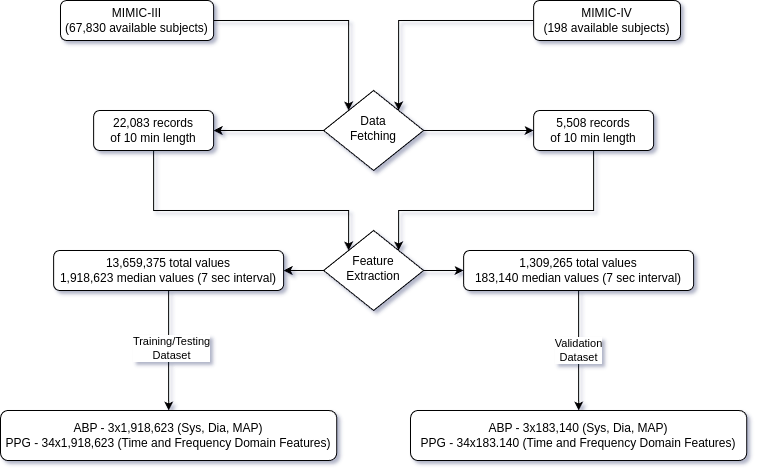
\includegraphics[width=0.9\textwidth]{images/results/flow_diagram}
    \caption{Flow Diagram presenting the Data Fetching and Processing}
    \label{fig:data_flow}
\end{figure}

\newpage

\subsection{Machine Learning}
\label{subsec:machine_learning}

Moving forward to the results stemming from the ML phase, the initial focus lies on the preparation of feature data.

As outlined in previous chapters, the intended split ratio of 60/20/20 for train/test/validation could not be precisely achieved due to the final dataset sizes of 1,918,623 values from MIMIC-III and 183,140 values from MIMIC-IV\@.
Consequently, the MIMIC-III dataset was utilized for training and testing, being split into an 80/20 ratio for train/test, resulting in 1,534,898 training datapoints and 383,725 testing datapoints.
Thus, the ultimate distribution for train/test/validate proportions became:

\begin{center}
    \begin{tabular}{|c|c|c|}
        \hline
        Training  & Testing & Validation \\
        \hline
        1,534,898 & 383,725 & 183,140    \\
        \hline
        73\%      & 18\%    & 9\%        \\
        \hline
    \end{tabular}
\end{center}

After implementing the 7 ML models outlined in the Methods section~\ref{subsec:ml_methods} and employing the described training method with an \enquote{early stopping} strategy,
along with validation on \enquote{unseen} simulated \enquote{real-world} (MIMIC-IV) data, a comprehensive set of performance metrics was compiled.
Firstly, the training and testing losses, measured through MSE at the conclusion of training epochs, were documented.
Secondly, the overall testing accuracy was assessed using RMSE and MAE metrics.
Lastly, the validation loss, also utilizing RMSE and MAE, was computed.

All \textit{PyTorch} models were additionally executed alongside their \enquote{weight adjusted} (WA) counterparts, with the respective metrics recorded.

The relevant ML model testing logs and performance metrics, including RMSE, MAE, \textit{$R^2$}, Bias and LoA are documented in Appendix~\ref{subsec:misc_measures}.

The plots depicting feature importance, along with their corresponding weight values from the second iteration of the ML models, are available in Appendix~\ref{subsec:plots_fi}.

The final results of all ML models for predicting ABP (SBP, DBP and MAP) are available in the Tables~\ref{tab:train_test_mse} and~\ref{tab:test_validate_rmse_mae}.

The validated prediction accuracy of different BP measurements across all ML models is illustrated in Figure~\ref{fig:all_mae}.

\subsubsection{Feature Importance}

Based on the iterative evaluation approach described in the methods section, the feature importance values were systematically analyzed, highlighting their impact on the model's performance.
The plots, available in the Appendix~\ref{subsec:plots_fi}, showcase these values in a descending order, revealing the features' contributions to either enhancing or diminishing the model's predictive power.
From the obtained results, a portion of the features can be categorized into three groups based on their average importance values.

In the category of best performers, features such as
\begin{itemize}
    \item Diastolic Time (86.89),
    \item Resistive Index (67.31),
    \item Diastolic + Systolic Width at 50\% (50.6) and
    \item Normalized Power at Peak (46.72)
\end{itemize}
stood out prominently, demonstrating significant influence in improving the models' accuracy.

In the medium-performing group, features like
\begin{itemize}
    \item Delta Area (37.12),
    \item Vessel Volume Systolic Index (23.61),
    \item Systolic Area and
    \item Total Power (both with values of 20.79), also
    \item Diastolic Width at 66\% (17.66) and
    \item Vessel Volume Diastolic Index (14.27),
\end{itemize}
contributed moderately to the overall predictive capability.

Lastly, in the category of least influential features
\begin{itemize}
    \item Mean Frequency (3.51)
    \item and Ratio of Diastolic to Systolic Width at 75\% (2.12)
\end{itemize}
showed minimal impact on the models' performance.

\subsubsection{Model Performance}

% Training loop
\begin{table}[p]
    \renewcommand{\arraystretch}{1.5}
    \begin{center}
        \footnotesize
        \begin{tabular}{ |c|c|c| }
            \hline
            & Training Loss (MSE)        & Testing Loss (MSE)          \\
            \hline
            LR           & \cellcolor{red!10}217.673  & \cellcolor{red!10}217.255   \\
            \hline
            LR (WA)      & \cellcolor{red!20}217.721  & \cellcolor{red!20}217.284   \\
            \hline
            MLP          & 196.448                    & 196.158                     \\
            \hline
            MLP (WA)     & \cellcolor{red!30}246.247  & \cellcolor{red!30}249.776   \\
            \hline
            LSTM         & \cellcolor{green!20}97.452 & \cellcolor{green!20}101.49  \\
            \hline
            LSTM (WA)    & 138.708                    & 143.316                     \\
            \hline
            Bi-LSTM      & \cellcolor{green!10}115.1  & 118.12                      \\
            \hline
            Bi-LSTM (WA) & 154.553                    & 159.745                     \\
            \hline
            GRU          & \cellcolor{green!30}89.809 & \cellcolor{green!30}93.605  \\
            \hline
            GRU (WA)     & 138.081                    & 142.129                     \\
            \hline
            Bi-GRU       & 115.506                    & \cellcolor{green!10}117.732 \\
            \hline
            Bi-GRU (WA)  & 117.547                    & 173.893                     \\
            \hline
        \end{tabular}
    \end{center}
    \captionsetup{format=plain, justification=centering, font=small}
    \caption{Training and Testing Losses of different ML models at the end of training}
    \label{tab:train_test_mse}
\end{table}

The results of the Machine Learning models, as summarized in Table~\ref{tab:train_test_mse} , reveal varying levels of performance in terms of training and testing losses at the conclusion of training epochs.
The intermediate training and testing losses are plotted in Figure~\ref{fig:train_test_mse}.

The LR model exhibited a training loss of 217.673 (MSE) and a testing loss of 217.255 (MSE), with marginal improvement seen in the \enquote{weight adjusted} (WA) version.
Similarly, the MLP model showed a training loss of 196.448 (MSE) and a testing loss of 196.158 (MSE), with a notable increase in losses for the WA variant.

On the other hand, the LSTM model demonstrated improved performance, showcasing a training loss of 97.452 (MSE) and a testing loss of 101.49 (MSE), while the Bi-LSTM and Bi-GRU models also exhibited relatively lower losses.
The GRU model, in particular, displayed a training loss of 89.809 (MSE) and a testing loss of 93.605 (MSE), indicating promising results for this configuration.

Overall, the models' performances varied, with some showing better generalization capabilities than others, as evident from their testing losses.

% Test and Validation measures
\begin{table}[p]
    \renewcommand{\arraystretch}{1.5}
    \begin{center}
        \footnotesize
        \begin{tabular}{ |c|c|c|c|c| }
            \hline
            & Test MAE                  & Test RMSE                  & Validation MAE             & Validation RMSE            \\
            \hline
            LR           & \cellcolor{red!10}11.091  & \cellcolor{red!10}14.739   & 13.171                     & \cellcolor{green!30}16.219 \\
            \hline
            LR (WA)      & \cellcolor{red!20}11.093  & \cellcolor{red!20}14.74    & 13.196                     & 16.257                     \\
            \hline
            MLP          & 10.567                    & 14.005                     & 14.096                     & 18.781                     \\
            \hline
            MLP (WA)     & \cellcolor{red!30}11.802  & \cellcolor{red!30}15.803   & \cellcolor{red!30}21.309   & \cellcolor{red!30}30.559   \\
            \hline
            LSTM         & \cellcolor{green!10}7.119 & \cellcolor{green!10}10.073 & 14.158                     & 18.005                     \\
            \hline
            LSTM (WA)    & 8.697                     & 11.971                     & 13.16                      & 16.311                     \\
            \hline
            Bi-LSTM      & 7.85                      & 10.868                     & 14.921                     & \cellcolor{red!10}18.892   \\
            \hline
            Bi-LSTM (WA) & 9.362                     & 12.638                     & \cellcolor{green!30}12.95  & \cellcolor{green!10}16.253 \\
            \hline
            GRU          & \cellcolor{green!20}6.823 & \cellcolor{green!20}9.674  & \cellcolor{red!20}15.304   & 19.5                       \\
            \hline
            GRU (WA)     & 8.658                     & 11.921                     & \cellcolor{green!10}13.106 & 16.358                     \\
            \hline
            Bi-GRU       & 7.844                     & 10.85                      & \cellcolor{red!10}15.222   & \cellcolor{red!20}19.141   \\
            \hline
            Bi-GRU (WA)  & 9.811                     & 13.186                     & \cellcolor{green!20}13.096 & \cellcolor{green!20}16.244 \\
            \hline
            RF           & \cellcolor{green!30}5.075 & \cellcolor{green!30}8.148  & 14.736                     & 18.105                     \\
            \hline
        \end{tabular}
    \end{center}
    \captionsetup{format=plain, justification=centering, font=small}
    \caption{Testing and Validation Performance Metrics of different ML models}
    \label{tab:test_validate_rmse_mae}
\end{table}

\vspace{0.2cm}

The Table~\ref{tab:test_validate_rmse_mae} provides an overview of the testing and validation performance metrics for the Machine Learning models employed.

For the LR model, the test MAE and RMSE were recorded as 11.091 and 14.739 respectively, with the validation MAE at 13.171 and RMSE at 16.219.
Similarly, the LR WA model exhibited comparable metrics with slightly higher validation MAE and RMSE values.

Moving to the MLP model, it displayed a test MAE of 10.567 and a test RMSE of 14.005, with the validation metrics showing an MAE of 14.096 and RMSE of 18.781.
The MLP WA model significantly increased the validation losses MAE and RMSE to 21.309 and 30.559 respectively, displaying the worst performance of all models.

In contrast, the LSTM model showed improved performance with a test MAE of 7.119 and a test RMSE of 10.073.
The validation metrics for LSTM were recorded as an MAE of 14.158 and RMSE of 18.005.
The Bi-LSTM model also exhibited relatively lower MAE and RMSE values for both test and validation sets.

The GRU model displayed a test MAE of 6.823 and a test RMSE of 9.674, with the validation MAE at 15.304 and RMSE at 19.5.
For the Bi-GRU model, the test MAE and RMSE were 7.844 and 10.85, while the validation MAE and RMSE were recorded as 15.222 and 19.141 respectively.
The weight-adjusted versions of these models generally improved upon their validation metrics, with the Bi-LSTM WA model performing the most effectively with 12.95 validation MAE\@.

Lastly, the RF model stood out with the lowest test MAE and RMSE of 5.075 and 8.148 respectively.
The validation MAE for RF was 14.736 and RMSE was 18.105, showcasing its strong predictive capabilities across both test and validation datasets.

The analysis reveals varying performances among the models, with the RF model demonstrating consistently strong predictive accuracy, especially notable in its lower MAE and RMSE values across both test and validation datasets.

\subsubsection{Prediction Performance of different BP measurements}

\begin{figure}[h]
    \centering
    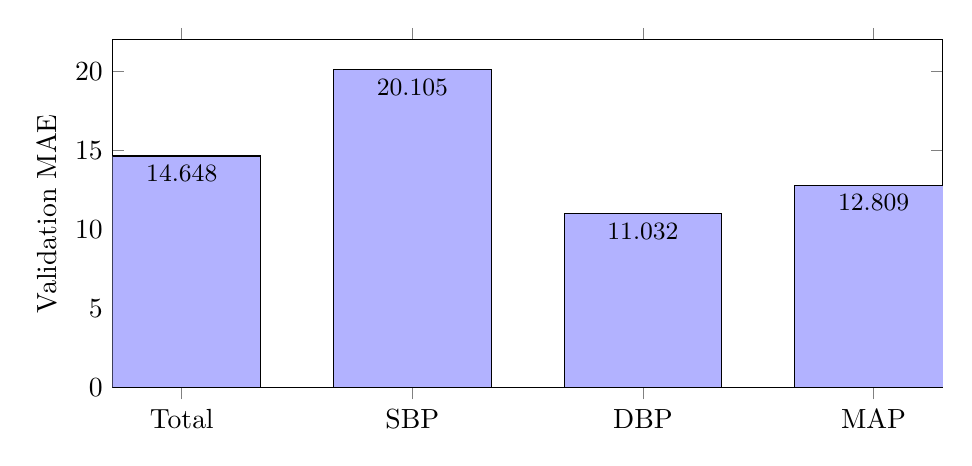
\begin{tikzpicture}
        \begin{axis}[
            width=\textwidth,
            height=6cm,
            ybar,
            ymin=0,
            ymax=22,
            bar width=2cm,
            xtick=data,
            xticklabels={Total, SBP, DBP, MAP},
            ylabel={Validation MAE},
            nodes near coords,
            nodes near coords style={font=\small, anchor=north, /pgf/number format/.cd, fixed, precision=3},
        ]
            \addplot[fill=blue!30] coordinates {(1,14.648) (2,20.105) (3,11.032) (4,12.809)};
        \end{axis}
    \end{tikzpicture}
    \captionsetup{format=plain, justification=centering, font=small}
    \caption{Average validation MAE of total, systolic, diastolic and mean arterial pressures}
    \label{fig:all_mae}
\end{figure}

The bar chart depicted in Figure~\ref{fig:all_mae} showcases the average validation MAE for distinct BP measurements.
Among the categories of Total, Systolic, Diastolic, and Mean Arterial Pressure, notable disparities in error levels were evident.

The overall average validation MAE, calculated across all models, was 14.648.
However, the individual measures displayed significant deviations.

Particularly, the most considerable MAE was observed for SBP at 20.105, indicating a pronounced level of error.
A substantial reduction in MAE was notable for DBP, nearly halving the error observed for SBP, with a recorded MAE of 11.032, marking the lowest among the measurements.
Meanwhile, MAP exhibited the second lowest MAE, closely trailing DBP at 12.809.

These findings offer valuable insights into the predictive performance of the model across distinct BP parameters,
with SBP presenting the highest margin of error, while DBP and MAP indicating relatively lower levels of error.

\begin{figure}[p]
    \centering
    \begin{minipage}{\textwidth}
        \centering
        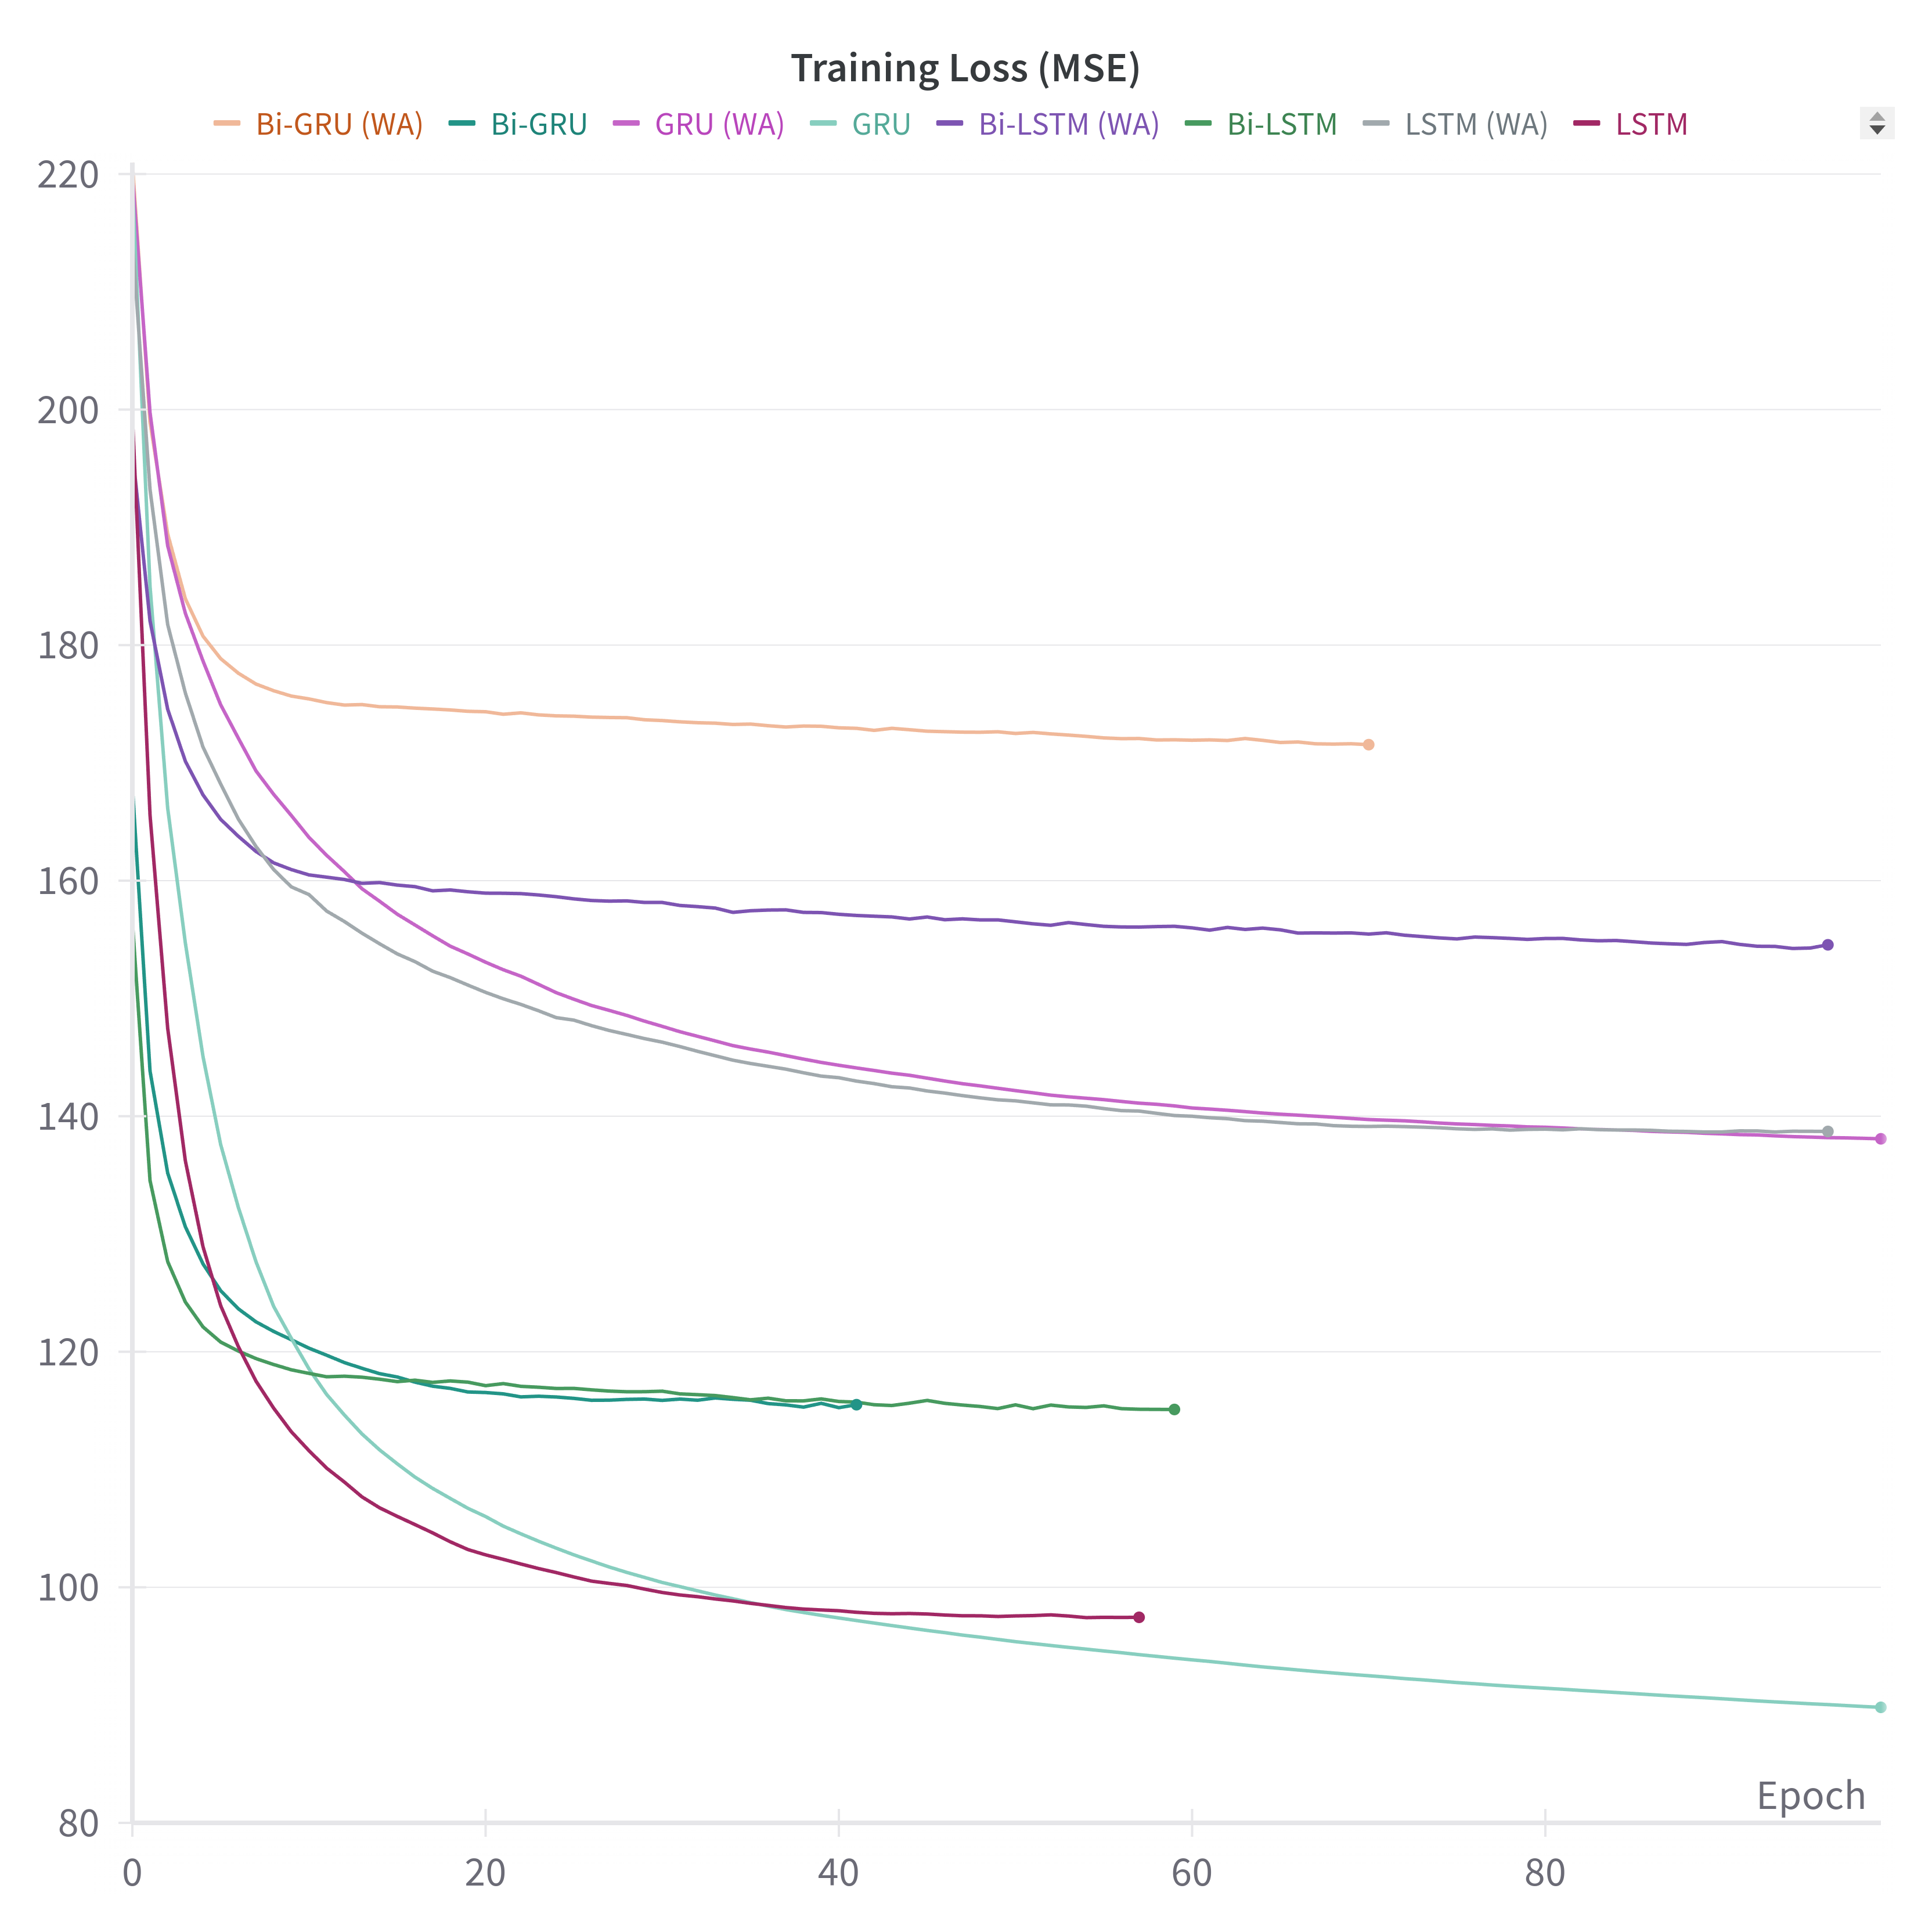
\includegraphics[width=0.7\textwidth]{images/results/training_loss_mse}
        \vspace{0.001cm}
        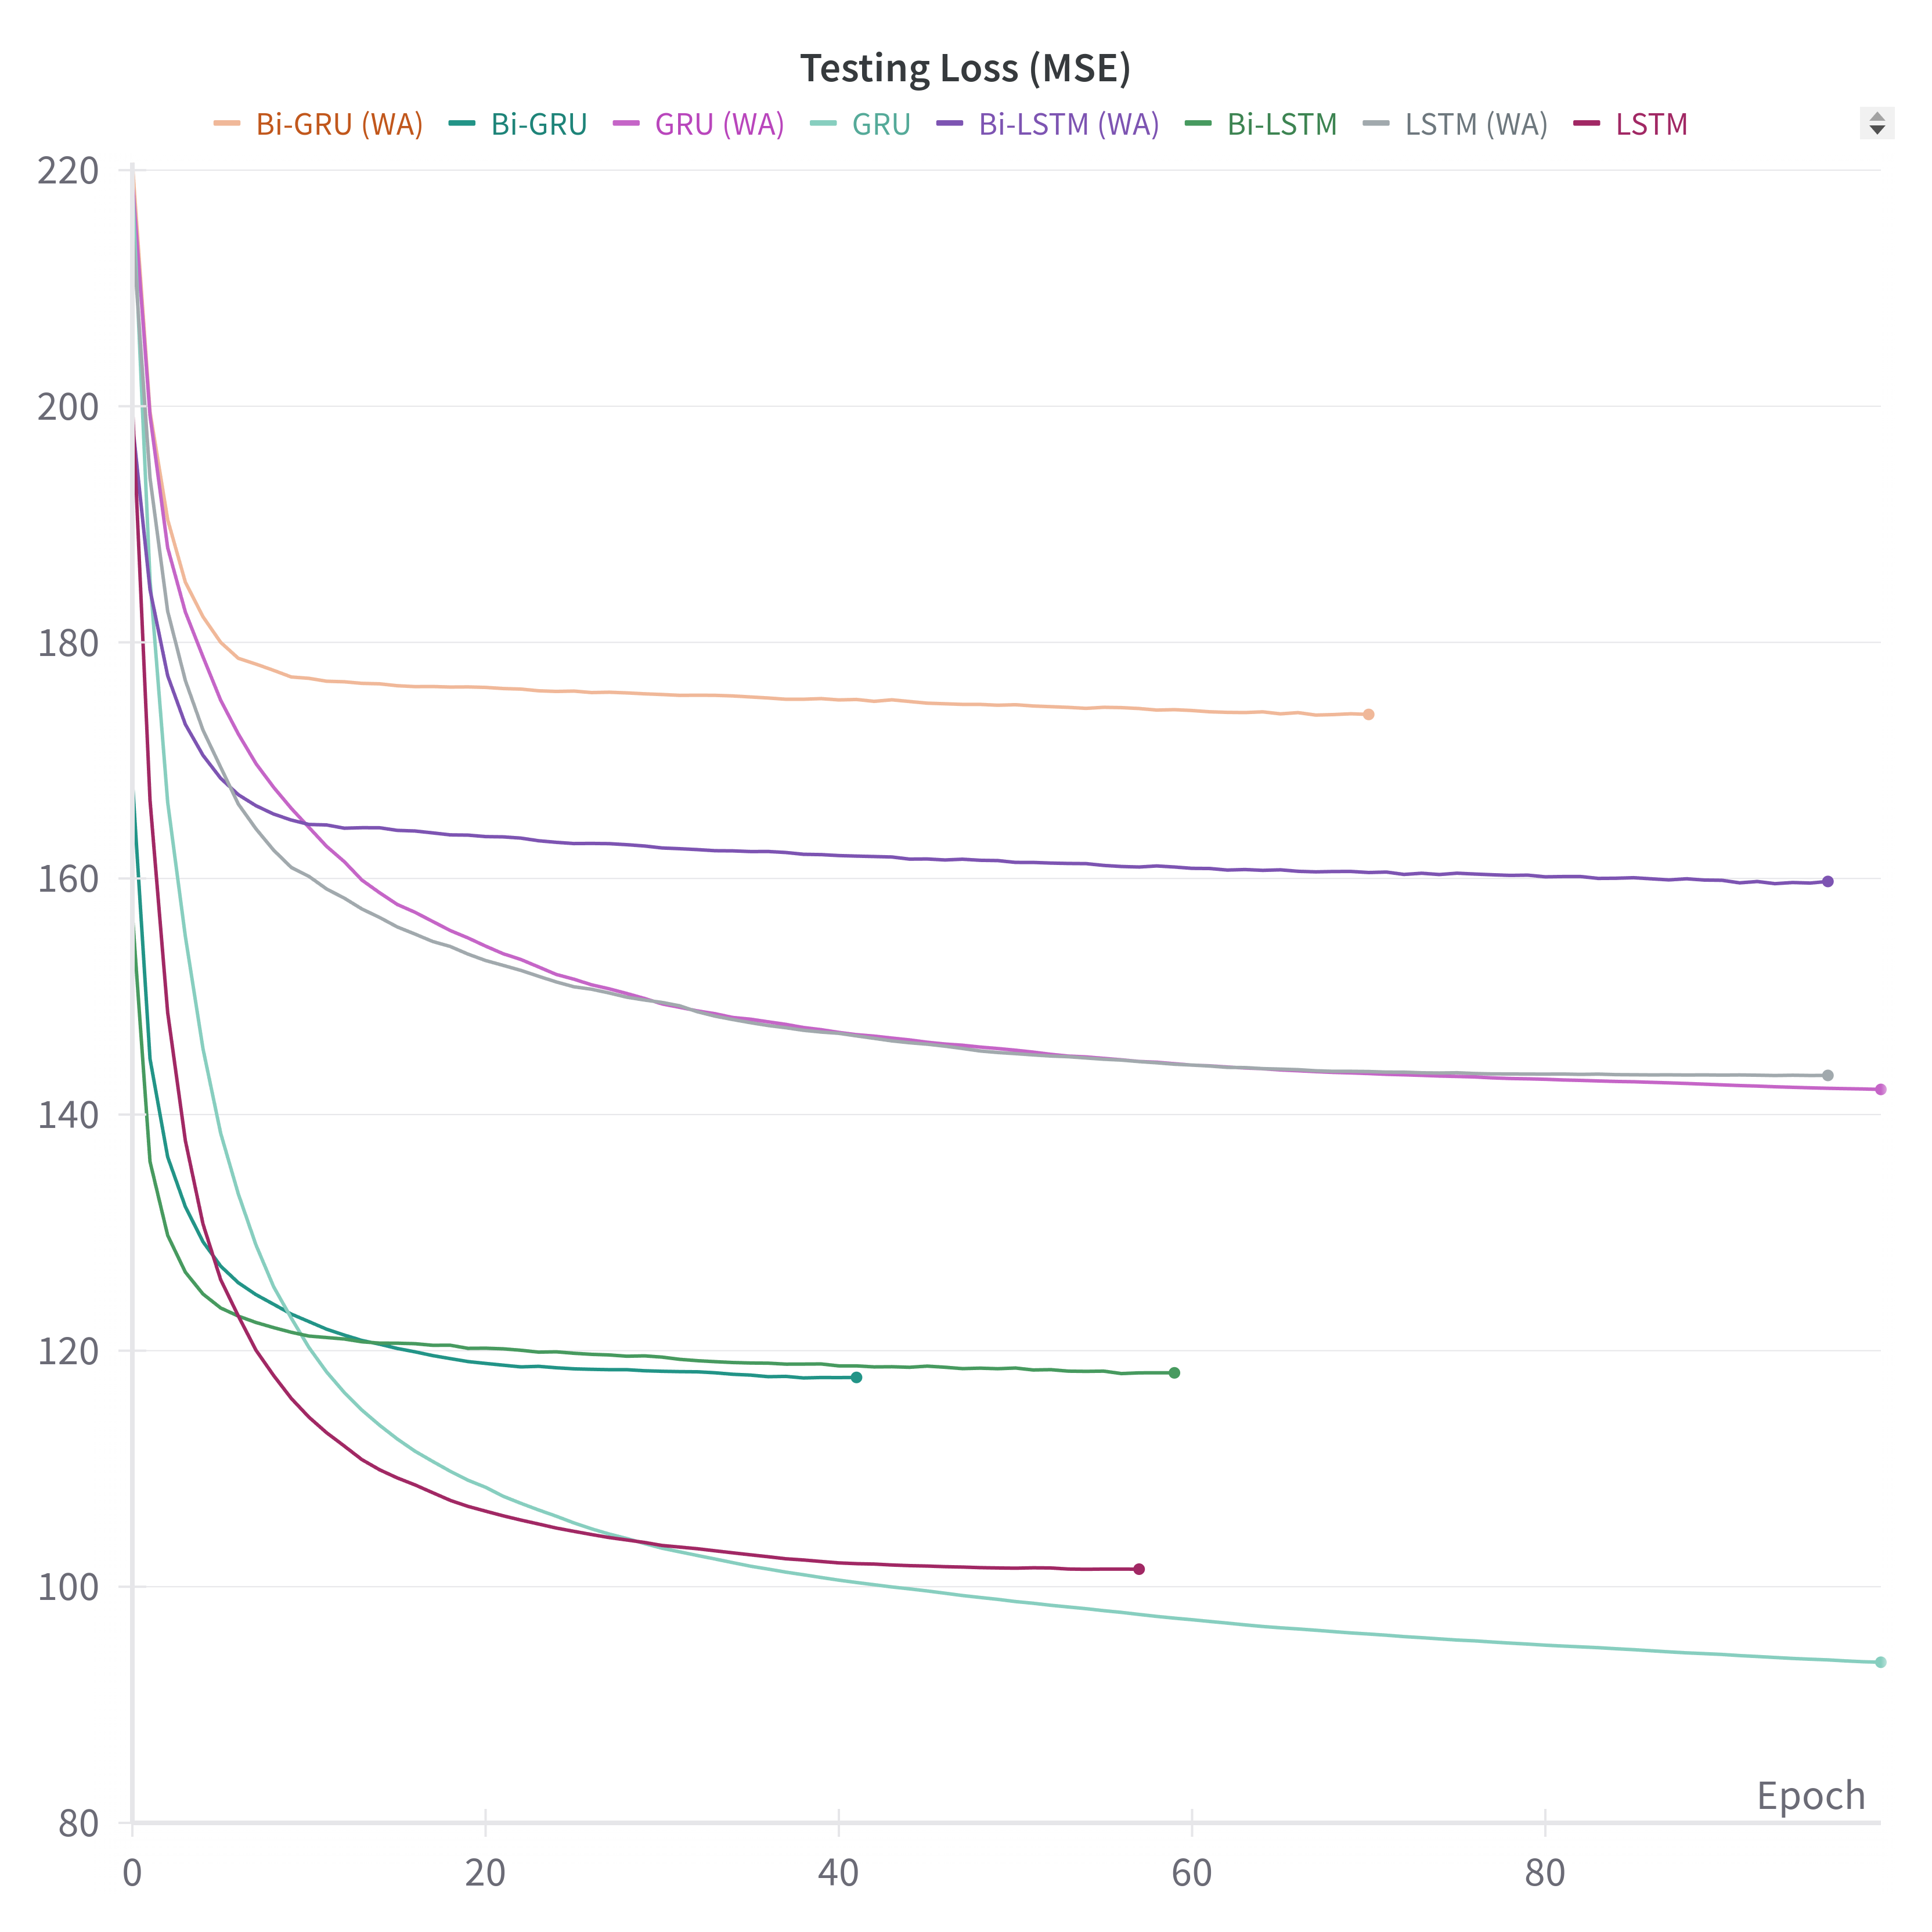
\includegraphics[width=0.7\textwidth]{images/results/testing_loss_mse}
        \captionsetup{format=plain, justification=centering, font=small}
        \caption{Training and Testing Losses of LSTM \& GRU Models}
        \label{fig:train_test_mse}
    \end{minipage}
\end{figure}

\newpage